%% ==========================================================================
%%  dgnozzle -- how two elements couple: traces, normal, numerical flux
%% ==========================================================================
\documentclass[tikz,border=6pt]{standalone}
\usepackage{amsmath}
\usetikzlibrary{arrows.meta,calc,decorations.markings}
\begin{document}

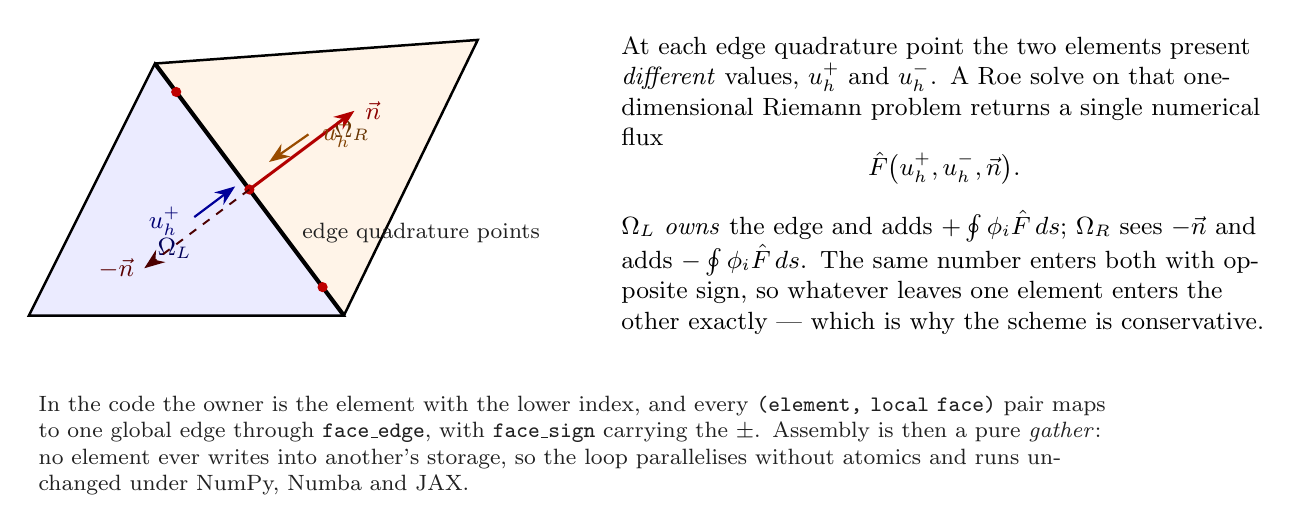
\begin{tikzpicture}[
  >={Stealth[length=2.6mm]},
  el/.style   = {line width=0.9pt},
  qp/.style   = {circle, fill=red!75!black, inner sep=1.3pt},
  lbl/.style  = {font=\small},
  slbl/.style = {font=\footnotesize, gray!25!black},
]

%% two triangles sharing an edge
\fill[blue!8]   (0,0) -- (4,0) -- (1.6,3.2) -- cycle;
\fill[orange!9] (4,0) -- (1.6,3.2) -- (5.7,3.5) -- cycle;
\draw[el] (0,0) -- (4,0) -- (1.6,3.2) -- cycle;
\draw[el] (4,0) -- (5.7,3.5) -- (1.6,3.2);

\draw[line width=1.5pt, black] (4,0) -- (1.6,3.2);

\node[lbl, blue!35!black]   at (1.85,0.85) {$\Omega_L$};
\node[lbl, orange!40!black] at (4.1,2.35)  {$\Omega_R$};

%% quadrature points on the shared edge
\foreach \t in {0.1127,0.5,0.8873}
  { \node[qp] at ($(4,0)!\t!(1.6,3.2)$) {}; }
\node[slbl, anchor=west] at (3.35,1.05) {edge quadrature points};

%% outward normal of the owner (L)
\coordinate (mid) at ($(4,0)!0.5!(1.6,3.2)$);
\draw[->, red!70!black, line width=1.1pt] (mid) -- ++(1.335,1.0)
      node[right, lbl, red!55!black] {$\vec{n}$};
\draw[->, red!30!black, line width=0.7pt, dashed] (mid) -- ++(-1.335,-1.0)
      node[left, lbl, red!35!black] {$-\vec{n}$};

%% traces
\draw[->, blue!60!black, line width=0.8pt] (2.1,1.25) -- (2.62,1.64);
\node[lbl, blue!45!black, anchor=east] at (2.05,1.2) {$u_h^{+}$};
\draw[->, orange!60!black, line width=0.8pt] (3.55,2.3) -- (3.05,1.95);
\node[lbl, orange!50!black, anchor=west] at (3.6,2.32) {$u_h^{-}$};

%% the Riemann problem
\node[lbl, align=left, anchor=west, text width=8.2cm] at (7.4,2.6)
  {At each edge quadrature point the two elements present
   \emph{different} values, $u_h^{+}$ and $u_h^{-}$.  A Roe solve on that
   one-dimensional Riemann problem returns a single numerical flux
   \[ \hat{F}\bigl(u_h^{+}, u_h^{-}, \vec{n}\bigr). \]};

\node[lbl, align=left, anchor=west, text width=8.2cm] at (7.4,0.55)
  {$\Omega_L$ \emph{owns} the edge and adds $+\oint \phi_i \hat{F}\,ds$;
   $\Omega_R$ sees $-\vec{n}$ and adds $-\oint \phi_i \hat{F}\,ds$.  The same
   number enters both with opposite sign, so whatever leaves one element
   enters the other exactly --- which is why the scheme is conservative.};

\node[slbl, align=left, anchor=north west, text width=13.8cm] at (0,-0.9)
  {In the code the owner is the element with the lower index, and every
   \texttt{(element, local face)} pair maps to one global edge through
   \texttt{face\_edge}, with \texttt{face\_sign} carrying the $\pm$.  Assembly is
   then a pure \emph{gather}: no element ever writes into another's storage, so
   the loop parallelises without atomics and runs unchanged under NumPy, Numba
   and JAX.};

\end{tikzpicture}

\end{document}
